\documentclass[12pt]{article}
\usepackage{graphicx}
\usepackage{amssymb}
\usepackage{epstopdf}
\usepackage{amsmath}
\usepackage{multicol}
\usepackage{tcolorbox}
\usepackage{geometry}
\usepackage{enumitem}
\usepackage{fancyhdr}
\usepackage{pifont,amssymb} % for the symbols

\newlist{todolist}{itemize}{2}
\setlist[todolist]{label=$\square$}


\textwidth = 6.5 in
\textheight = 9 in
\oddsidemargin = 0.0 in
\evensidemargin = 0.0 in
\topmargin = -23pt
\headheight = 0.0 in
\headsep = 0.0 in
\parskip = 0.2in
\parindent = 0.0in
\pagestyle{fancy}
\pagenumbering{gobble}

\newtheorem{theorem}{Theorem}
\newtheorem{corollary}[theorem]{Corollary}
\newtheorem{definition}{Definition}
%\includegraphics [height=50mm, width=50mm]{PathInt.jpg}
\title{Title} 

\begin{document}
%INSTRUCTOR NOTES

 Name:
 \begin{center}\large{3.9 Linear Approximation}\end{center}

\begin{enumerate}
\item Write the equation for the line tangent to $f(x) = 3\sqrt{x-1} - 2$ at $x = 5$.

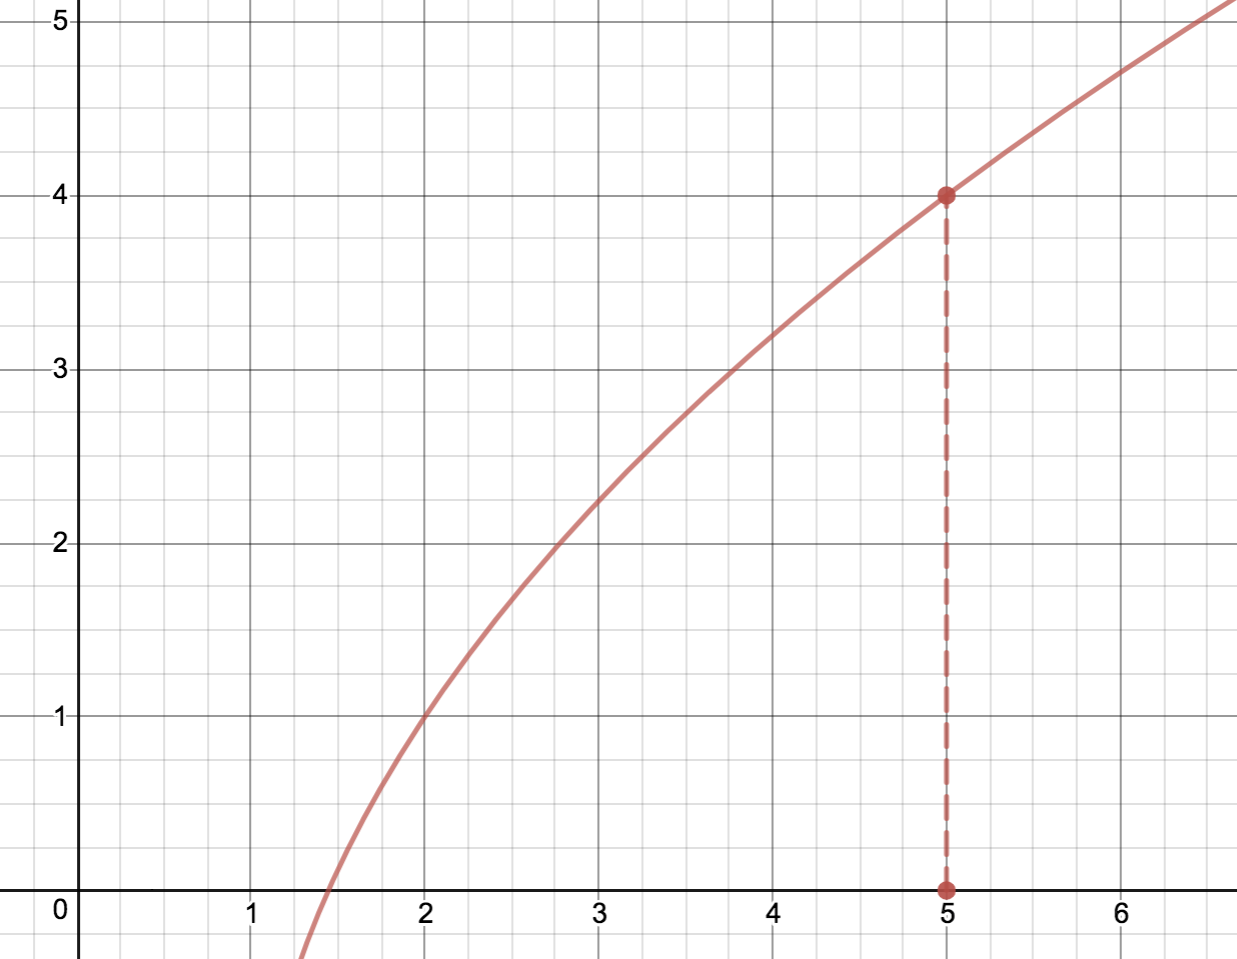
\includegraphics[width=2.5in]{3_9_linear1.png}

\begin{tcolorbox}
\textbf{Definition:} The Equation for a tangent line to the function $f(x)$ at the point $(a,f(a))$ with slope $f'(a)$ is
$$L_a(x) = f'(a)(x-a) + f(a)$$

Note: $f(a)$ and $f'(a)$ are NUMBERS

All functions which are \textit{locally linear} at $x=a$ are differentiable at $x=a$. Also, all functions which are differentiable at $x=a$ are locally linear at $x=a$. A function is \textit{locally linear} if ....

$\hspace{10px}$ \\

\end{tcolorbox}

\item Let $f(x) = \frac{1}{2} (x-2)^3 + 3$.

	\begin{enumerate}
	\item Find the equation for the linear approximation of $f$ at $x=3$.
		$$L(x) = $$
		
	\item Add a few more x-values to the table below and compare the outputs of the original function and the tangent line approximation.
	
		\begin{tabular}{l||l|l|l}
		$x_1$ & $f(x_1)$ & $L(x_1)$ & $L(x_1) - f(x_1)$ \\ \hline
		$3$   & $3.5$    &          &                   \\
		      &          &          &                   \\
		      &          &          &                  
		\end{tabular}
		
	\item How good is the linear approximation at estimating the actual value of the function?
	\vfill
		
	\end{enumerate}

\newpage

$\hspace{10px}$ \\

\begin{tcolorbox}
\textbf{Definition:} The error is the difference between the actual value (given by $f$), and the approximate value (given by $L$), with equation

$$E(x) = f(x) - L(x) = $$

For a nicely behaved function,

$$E(x) \approx \frac{f''(a)}{2} (x-a)^2$$
\end{tcolorbox}

\item Use the function $f(x) = \sqrt[5]{x}$ and its tangent line at $x=1$ to estimate the fifth root of $2$ without using your calculator. Is this an over estimate or an under estimate?
\vfill

\item If $h(0) = 4$ and $h'(0) = -5$, use a linear approximation to estimate $h(0.25)$.
\vfill

\item Given that $g$ is continuous, differentiable, and contains the value given in the table, estimate $g(3.2)$.

		\begin{tabular}{l||l|l|l|l}
		$x$ & $-\frac{3}{2}$ & $\frac{5}{2}$ & $3$ & $7$ \\ \hline
		$g(x)$   & $6$    &  $-\frac{7}{4}$   & $-\frac{1}{2}$ & 14.3                  \\     
		\end{tabular}
\vfill

\end{enumerate}

\end{document} 
